%# -*- coding: utf-8-unix -*-
\chapter{基于眼动数据的立体图像质量评价模型}
\label{chap:model}
通过前面的工作,我们已经得到了预处理过的眼动数据和主观评分数据集$Q$。这部分我们来利用眼动数据评价立体图像质量。由于眼动数据具有量大、无直接规律的特点,我们首先特征提取,然后与主观评分拟合。在这方面,SVR\parencite{scholkopf2000new}被常用来建立回归模型。本文的工作将从以下四个方面展开:
\begin{itemize}[noitemsep,topsep=0pt,parsep=0pt,partopsep=0pt]
\item 首先,结合前人研究成果和生理学知识,提取眼动特征;
\item 然后,将提出的特征集随机地分为训练集$\phi _1$与预测集$\phi _2$两部分,其中训练集占80\%,预测集占20\%,利用SVR回归模型训练眼动特征和主观评分MOS值获取“模型”,如图\ref{fig:train:a}。假设一副图像$I{}_i $对应的眼动数据数据特征为$f^i=\{f_1^i,f_2^i,...f_n^i\}$,则SVR训练过程可以表示为
\begin{equation}
model = SVR\_TRAIN([{f_j^i}],[{q_i}])\qquad I{}_i \in {\phi _1},j \in [1,n]
\end{equation}
\item 再次,用预测集作为“model”的输入,则相应地输出就是该图像对应的预测主观评分值,如图\ref{fig:predict:b},可以表示为
\begin{equation}
s_i = SVR\_PREDICT([{f_j^i}],model])\qquad I{}_i \in {\phi _2},j \in [1,n]
\end{equation}
\item 最后,选用PLCC、SROCC以及RMSE来衡量预测值与实际值之间的相关性和精度,从而得出结论。
\end{itemize}

\begin{figure}
  \centering
  \subfigure[SVR训练过程]{
    \label{fig:train:a} %% label for first subfigure
    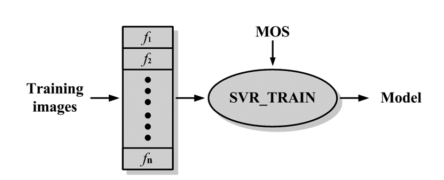
\includegraphics[width=0.48\textwidth]{chap5/train.png}}
  \hspace{0.2in}
  \subfigure[SVR预测过程]{
    \label{fig:predict:b} %% label for second subfigure
    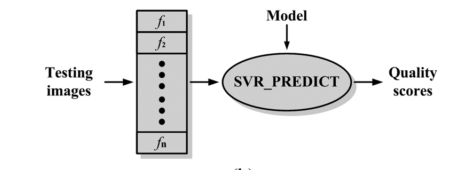
\includegraphics[width=0.48\textwidth]{chap5/predict.png}}
  \bicaption[fig:SVR]{SVR回归模型过程,图a为SVR训练示意图,图b为SVR预测示意图}{SVR回归模型过程\supercite{gu2015using}}{Fig}{The procedure of SVR}
\end{figure}

\section{眼动特征的提取}
\label{sec:featureextract}
首先,从眼动数据的时序特征开始。张\parencite{zhang2014application}从时序的角度分析了人眼观看2D视频和3D视频过程中的运动差异,采用的主要指标包括眨眼频率、眨眼持续时间、注视持续时间、瞳孔直径、眼跳速度与加速度、眼跳持续时间、眼跳幅度。由于其已经得出了一些很有价值的结论,所以本文将从眼动数据中提取这些指标作为特征。

我们先从眨眼的特征开始,眼睛眨眼的过程在眼动数据中主要表现为两只眼睛在连续的时间内不能被捕捉到,且持续一定的时间。眼睛眨眼在眼动数据中可以描述为:
\begin{equation}
\left\{ \begin{array}{l}
lefteyestate = 4\\
righteyestate = 4
\end{array} \right.\
\end{equation}
这里$lefteyestate=4,righteyestate=4$分别表示左右眼在测量时刻未被测量到。在具体操作中,将该状态的持续时间设定为1/15s(1s测量60次,眨眼的过程至少要连续占4个采样点),防止眼动数据的误测。由于每个人测量的时长均设定成了10s,因此,眨眼频率与眨眼个数是等价的。眨眼的持续时间则是所有眨眼过程持续时间总和。眨眼时间和眨眼频率的特征可以描述为(如无特殊说明,则下列所有特征都是针对所有人对图像$I_i$的观看评价结果):
\begin{equation}
{f_1^i} = \frac{1}{n}\sum\limits_{k = 1}^n {{b_{i,k}}} 
\end{equation}
这里${b_{i,k}}$表示第$k$个人看第$i$副图像时产生的眨眼个数。
\begin{equation}
{f_2^i} = \frac{1}{n}\sum\limits_{k = 1}^n {{t_{i,k}}} 
\end{equation}
这里${t_{i,k}}$表示第$k$个人看第$i$副图像时眨眼持续的时长。

在第\ref{chap:dataprocess}章,我们对眼动数据进行了预处理,通过滤波可以分离出眼动数据的注视点和扫视点。因为人眼在观看图像时获取信息最重要的眼动过程是注视过程,Kim\parencite{kim2014saliency}的工作表明不同舒适性的图像对应的注视区域特征不同:舒适度高的图片注视区域相对来说比较集中,而舒适度低的图像对应的注视区域相对比较分散,如图\ref{fig:kimresult}。也就是说,质量高的图片由于注视区域集中,注视点持续时间较长,那么注视点个数就比较少,质量差得图片则相反。假设该结论正确,这里针对注视点提取三个特征:注视点个数,注视点持续时间均值,注视点持续时间最大值。
\begin{equation}
{f_3^i} = \frac{1}{n}\sum\limits_{k = 1}^n {{\eta _{i,k}}} 
\end{equation}
这里${\eta _{i,k}}$表示第$k$个人看第$i$副图像时注视点的个数。
\begin{equation}
{f_4^i} = \frac{1}{n}\sum\limits_{k = 1}^n {\mathop {\max }\limits_{1 \le j \le num} ({\eta _{i,k,j}})} 
\end{equation}
\begin{equation}
{f_5^i} = \frac{1}{n}\sum\limits_{k = 1}^n {\sum\limits_{j = 1}^{num} {{\eta _{i,k,j}}} } 
\end{equation}
这里${\eta _{i,k,j}}$表示第$k$个人看第$i$副图像时的第$j$个注视点,$num$表示注视点个数。
\begin{figure}[!htp]
  \centering
  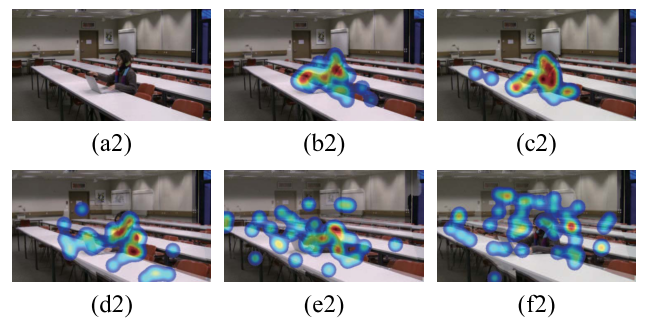
\includegraphics[width=0.8\textwidth]{chap5/kimresult.png}
  \bicaption[fig:kimresult]{Kim实验的结果,${a_2}$是原图,${b_2}$---${f_2}$为舒适性逐渐降低的图像对应的注视点热度图}{Kim实验的结果,${a_2}$是原图,${b_2}$---${f_2}$为舒适性逐渐降低的图像对应的注视点热度图\supercite{kim2014saliency}}{Fig}{Kim's result\supercite{kim2014saliency},${a_2}$ is original image and ${b_2}$---${f_2}$ are the density maps for images with decreased comfort.}
\end{figure}

在\ref{sec:singleye}节中提到了瞳孔在视觉生理过程中的作用,它可以调节进入眼睛的光的量。因此,瞳孔在不同注视区域下的直径是变化的,而且\parencite{zhang2014application}也将瞳孔直径作为了指标,所以这里提出关于瞳孔直径的两个特征。
\begin{equation}
\label{eq:f6}
{f_6^i} =\frac{1}{n}\sum\limits_{k = 1}^n {(\frac{1}{m}\sum\limits_{t = 1}^m {LP{D_{i,k,t}}} } )
\end{equation}
\begin{equation}
\label{eq:f7}
{f_7^i} = \frac{1}{n}\sum\limits_{k = 1}^n {(\frac{1}{m}\sum\limits_{t = 1}^m {RP{D_{i,k,t}}} } )
\end{equation}
其中${LP{D_{i,k,t}}}$,${RP{D_{i,k,t}}}$分别表示第$k$个人在看第$i$副图像时$t$时刻的左右眼直径,m表示当前图像在当前被试观看下的采样点。
特征\ref{eq:f6},\ref{eq:f7}是第$i$副图像的所有观看者的左右眼瞳孔均值。

人眼的立体视觉原理告诉我们,人眼对现实世界产生深度感来源于两个眼睛看到略有差异的事物,这种差异被描述为视差,因此,视差是立体成像的重要因素。在前面的综述\ref{sec:eyetrackapplied3D}中,我们提到了Liu\parencite{liu2010dichotomy}和Kim\parencite{kim2014saliency}都利用眼动数据对立体图像的视差进行了研究并得出了相关结论。事实上,图\ref{fig:kimresult}的不同的舒适性就是由同一图像进行不同的视差变化得到的。
眼动数据作为眼睛运动过程的记录,自然包含眼睛在观看图像的过程中蕴含的视差信息。利用\ref{sec:caldisparity}中提到的视差角计算方法,可以得到观看图像时的所有视差角信息。眼动数据的视差角信息和立体图像质量之间是否存在关联呢?这里提出一些与视差角相关的特征来进行验证。

首先来看视差角的总体特征,总体考虑整个观看过程,计算所有有效记录的相应视差角值,然后将视差角均值
\begin{equation}
\label{eq:f8}
{f_8^i} =\frac{1}{n}\sum\limits_{k = 1}^n {(\frac{1}{m}\sum\limits_{t = 1}^m {{d_{i,k,t}}} )} \qquad({d_{i,k,t}} \in D = \{ {d_{i,k,t}},t \in R\} ) 
\end{equation}
和方差
\begin{equation}
\label{eq:f9}
{f_9^i} =\frac{1}{n}\sum\limits_{k = 1}^n {(\sqrt {\frac{1}{m}\sum\limits_{t = 1}^m {({d_{i,k,t}} - \overline {{d_{i,k}}} } } )^2}  \qquad({d_{i,k,t}} \in D = \{ {d_{i,k,t}},t \in R\} )
\end{equation}
设定为相应特征。这里${d_{i,k,t}}$表示第$k$个人在看第$i$副图像时$t$时刻的视差角,$R$表示未分离眼动过程的原始序列(Raw Data),$D$是与$R$对应的视差角的集合。(下同)

前面提到,整个观看过程包含了注视、扫视、眨眼等过程,而注视过程是获取信息的核心部分,因此,注视阶段在整个观看过程中占有较大的比重是合理地,这里只关注注视阶段的视差角,提取均值作为其特征。
\begin{equation}
\label{eq:f10}
{f_{10}^i} =\frac{1}{n}\sum\limits_{k = 1}^n {(\frac{1}{m}\sum\limits_{t = 1}^m {{d_{i,k,t}}} )}   \qquad({d_{i,k,t}} \in D_f = \{ {d_{i,k,t}},t \in F\} )
\end{equation}
这里$F$表示分离眼动过程后注视区域对应的序列,$D_f$为与$F$对应的视差角。(下同)

在\ref{sec:densitymap}中进行了立体图像的眼动数据的分层表示,发现以视差角分割后,大部分注视点的集中在“小”视差角区域,即视差角绝对值较小的部分。因此,一个很有意思的问题是当视差角处于哪一层时与立体图像质量更为密切?考虑到不同图像的分层数量并不相同,所以以处于某个区域的视差角来代替。这里通过实验来确定该视差角区域。

首先以视差角的绝对值的大小进行升序排列,假设前$x\%$的视差角与立体图像质量有关联。取前$x\%$的视差角的均值与已知的MOS值进行拟合。当相关系数最大时,则当前的$x$为临界值。所以,构造以百分比$x$为横轴,以线性相关系数为纵轴的函数:
\begin{equation}
H(x) = LCC(\frac{1}{n}\sum\limits_{k = 1}^n {E(\{ {d_{i,k,t}}\} ),S)\qquad({d_{i,k,t}} \in D,S = \{ MO{S_i}\},t \in R )} 
\end{equation}
其结果如图\ref{fig:relationshipbetweenpercentandmos}所示:
\begin{figure}[!htp]
  \centering
  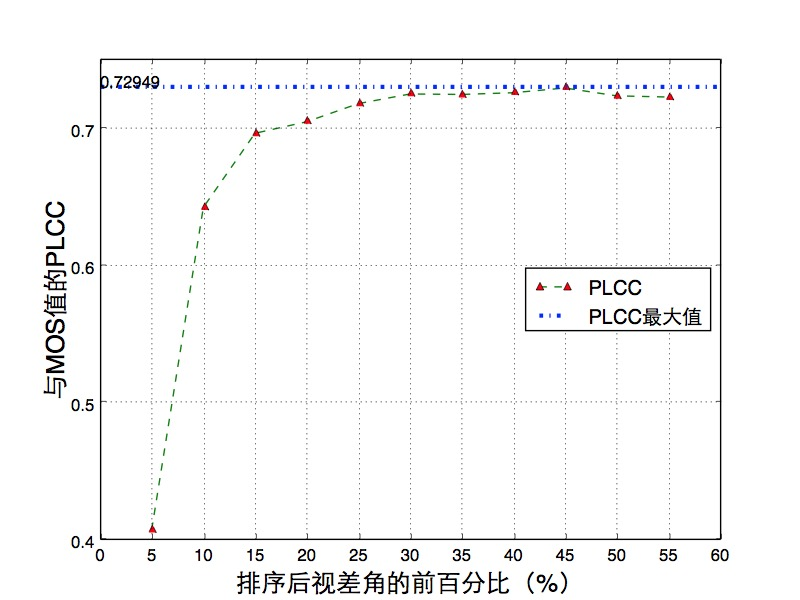
\includegraphics[width=0.75\textwidth]{chap5/relationshipbetweenpercentandmos.jpg}
  \bicaption[fig:relationshipbetweenpercentandmos]{前百分之$x$的视差角均值与MOS值的相关系数}{前百分之$x$的视差角均值与MOS值的相关系数(\%)}{Fig}{The relationship between percent x and mos}
\end{figure}

从图中可以看出,随着视差角百分比的提高,其与MOS值的相关系数逐步增大,当$x=45$时相关系数达到最大。因此我们采用按绝对值大小升序排列后的前45\%的视差角均值作为特征
\begin{equation}
\label{eq:f11}
{f_{11}^i} = \frac{1}{n}\sum\limits_{k = 1}^n {(\mathop E\limits_{t \in F} (\{ {d_{i,k,t}}\} ))} ({d_{i,k,t}} \in [top{\rm{ }}\ x] \subseteq F')
\end{equation}
这里$F'$是注视区域按视差角绝对值升序排列的视差角集合。同理,用$F''$表示注视区域按视差角绝对值降序排列的视差角集合。采用按绝对值大小降序排列后的前45\%的视差角均值作为特征
\begin{equation}
\label{eq:f12}
{f_{12}^i} = \frac{1}{n}\sum\limits_{k = 1}^n {(\mathop E\limits_{t \in F} (\{ {d_{i,k,t}}\} ))} ({d_{i,k,t}} \in [top{\rm{ }}\ x] \subseteq F'')
\end{equation}
\begin{figure}[!htp]
  \centering
  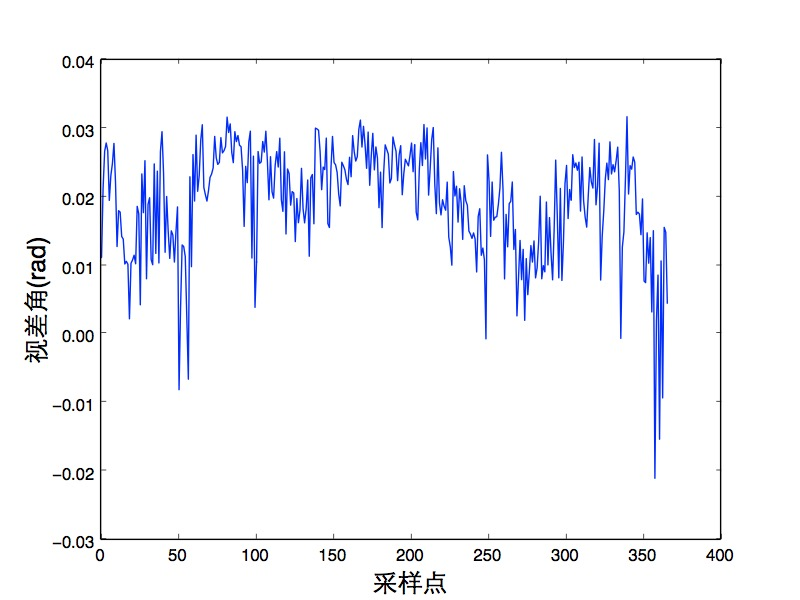
\includegraphics[width=0.75\textwidth]{chap5/disparitysample.jpg}
  \bicaption[fig:disparitysample]{视差角变化示意图}{视差角变化示意图}{Fig}{The disparity angular example}
\end{figure}
从眼动的过程来看(如图\ref{fig:disparitysample}),视差角的大小一直从大到小,从正到负的变化中,这种变化既是眼睛自身因素(如眼颤等)引起的结果,也有立体深度变化引起的因素。因此,我们将视差角的梯度均值定义为一个特征。
视差角均值可以定义为:
\begin{equation}
\label{eq:f13}
\nabla {d_{i,k,t}} = {d_{i,k,t}} - {d_{i,k,t - 1}}
\end{equation}
梯度特征定义为梯度的均值
\begin{equation}
{f_{13}^i}  = \frac{1}{n}\sum\limits_{k = 1}^n {(\mathop E\limits_{t \in D} (\{ \nabla {d_{i,k,t}}\} ))}
\end{equation}
张\parencite{zhang2015visual}等人已经证明,当立体图像中存在多个显著性区域,且这些区域存在一定的深度差时,人眼在观看时会因为辐辏调节产生视觉疲劳,从而降低对立体图像的评分。在\ref{sec:filter}中,通过对眼动数据进行滤波,得到了观看过程中得注视点,时域上相邻的两个的注视点间会产生一次跳变,利用跳变前后的视差角之差来衡量跳变过程中得辐辏变化程度,因此定义两个特征——辐辏调节最大值和辐辏调节均值。需要说明的是这两个特征值在总体眼动数据中受异常值的影响没有意义,但是在已估计出的注视点间是有意义的,因为注视点是持续稳定的。
\begin{equation}
{f_{14}^i}  =  \frac{1}{n}\sum\limits_{k = 1}^n {(\mathop E\limits_{t \in F} (\{ \nabla {d_{i,k,t}}\} ))}\end{equation}
\begin{equation}
{f_{15}^i}  = \frac{1}{n}\sum\limits_{k = 1}^n {(\mathop {\max }\limits_{t \in F} (\{ \nabla {d_{i,k,t}}\} ))}\end{equation}

至此,我们从眼动数据的空间域和视差域提取了16个特征,这些特征包括了注视点相关特征,扫视过程特征,还有瞳孔变化特征,既有全体数据的特征,也有只包括注视过程的特征。我们将在下一部分来建立基于眼动数据特征的立体图像质量评价模型。
\section{基于SVR回归的图像质量评价模型}
\label{sec:modelconstruction}
获取眼动数据特征以后,我们来基于SVR建立模型。先来回顾一下已经获取的数据集:
\begin{itemize}[noitemsep,topsep=0pt,parsep=0pt,partopsep=0pt]
\item 77副立体图像$I=\{I_i\}$;
\item 77个与每幅图像对应的眼动数据特征集$f=\{f_j^i\}$
\item 77副图像对应的MOS值$Q =\{q_i\}$
\end{itemize}
其中$i \in [1,77]$,表示图像索引,$j \in [1,15]$,表示特征索引
我们利用Python版本实现的scikit-learn\footnote{\url{http://scikit-learn.org/stable/index.html}}库来做SVR拟合,首先构建统一的用于拟合的数据集
\begin{equation}
\Phi  = \{ [{f_j^i}],{q_i},{{\rm{I}}_i} \in I,j \in [1,n]\} {\rm{  }}
\end{equation}
$\Phi $共包含77条记录,每条记录由对应于一副图像的特征集和MOS值组成。

利用随机发生器,将$\Phi $分为训练集$\phi _1$与预测集$\phi _2$
\begin{equation}
\Phi  = {\phi _1} \cup {\phi _2}
\end{equation}
其中训练集$\phi _1$包含60条记录,预测集$\phi _2$包含17条记录。

SVR回归模型有三种内核,分别为线性核、多项式核以及径向基内核。假设训练集为${({x_i},{y_i} \in {R^d},i = 1, \ldots ,n)}$。则三种核函数可以表示为:
\begin{itemize}[noitemsep,topsep=0pt,parsep=0pt,partopsep=0pt]
\item 线性核:
\begin{equation}
{k(x,y) = \left\langle {x,y} \right\rangle  + c = {x^T}y + c }
\end{equation}
\item 多项式核:
\begin{equation}
{k(x,y) = {(a\left\langle {x,y} \right\rangle  + c)^d} = {(a{x^T}y + c)^d}}
\end{equation}
\item 径向基内核
\begin{equation}
{k(x,y) = {e^{ - \gamma {{\left\| {x - y} \right\|}^2}}}}
\end{equation}
\end{itemize}

我们将对这几个内核都进行验证。其中多项式内核验证3次方的情况。
关于SVR,还有很重要的两个参数C和gamma,直接利用LibSVM库中的检测方法得出在我们的测试集下最优的C=2000,gamma=0.1.

做好这些准备后,现在开始训练,以MOS值作为标签,特征集为训练特征。获取模型后,利用预测集和模型,得到预测的主观评分,然后利用其与预测集实际的MOS值求PLCC,SROCC,RMSE。

为了保证测试结果的稳定性,我们将上述回归训练预测的过程重复1000次,然后取PLCC,SROCC,RMSE的均值作为最后的结果。整个过程可以表示为算法\ref{algo:svrprocedure}:

\begin{algorithm}
  \caption{SVR训练过程算法}
 \label{algo:svrprocedure}
  \begin{algorithmic}[1]
    \STATE initialize PLCC,SROCC,RMSE as empty list;
    \FOR{each $i$ in $[1,1000]$}
  	\STATE randlist = $random$(77);\
	\STATE $\phi _1$ = $\Phi $(randlist[1:60]);\
	\STATE $\phi _2$ = $\Phi $(randlist[60:77]);\
	\STATE $model$ = SVR\_TRAIN($\phi _1$);\
	\STATE $s_i$ = SVR\_PREDICT($\phi _2$,$model$);\
	\STATE plcc,srocc,rmse = Peasoncor($[s_i]$,$[q_i]$),Spearman($[s_i]$,$[q_i]$),Rmse($[s_i]$,$[q_i]$);\
	\STATE PLCC.append(plcc),SROCC.append(srocc),RMSE.append(rmse);   
    \ENDFOR
    \RETURN mean(PLCC),mean(SROCC),mean(RMSE);
  \end{algorithmic}
\end{algorithm}

最后,本文还考虑了基于不同眼睛滤波的情况。在\ref{sec:filter}中我们给出了眼动过程的滤波算法,我们知道传统的2D滤波是以双眼的平均位置为参考进行滤波的,而在3D场景,双眼是分工协作的,即人眼可以分为主眼与辅眼,主眼负责控制方向,辅眼则辅助产生深度。所以在滤波时可以选取不同的参考眼睛进行滤波。这里分别以左、右眼为参考进行了滤波。在提取特征时,共考虑了四种情况:分别从左眼、右眼、主眼、辅眼为参考的数据中提取特征。然后分别用三种核函数去做拟合。得到了模型训练的结果如下。
\begin{itemize}[noitemsep,topsep=0pt,parsep=0pt,partopsep=0pt]
\item 以从左眼为滤波参考的眼动数据中提取的特征训练预测的结果如表\ref{svrresultbasedonleft};
\begin{table}[]
\centering
\caption{从以左眼为参考滤波的数据中提取眼动特征的结果}
\label{svrresultbasedonleft}
\begin{tabular}{@{}cccc@{}}
\toprule
Kernel Type & PLCC              & SROCC             & RMSE              \\ \midrule
Linear      & \textbf{0.737874} & \textbf{0.671718} & \textbf{0.388042} \\
Poly        & 0.55636           & 0.511019          & 0.572146          \\
Rbf         & \textbf{0.734132} & \textbf{0.665892} & \textbf{0.398787} \\ \bottomrule
\end{tabular}
\end{table}
\item 以从右眼为滤波参考的眼动数据中提取的特征训练预测的结果如表\ref{svrresultbasedonright};
\begin{table}[]
\centering
\caption{从以右眼为参考滤波的数据中提取眼动特征的结果}
\label{svrresultbasedonright}
\begin{tabular}{@{}cccc@{}}
\toprule
Kernel Type & PLCC              & SROCC             & RMSE              \\ \midrule
Linear      & 0.699401          & 0.63249           & \textbf{0.408184} \\
Poly        & 0.556037          & 0.526174          & 0.576652          \\
Rbf         & \textbf{0.713655} & \textbf{0.650987} & 0.42011           \\ \bottomrule
\end{tabular}
\end{table}
\item 以从主眼为滤波参考的眼动数据中提取的特征训练预测的结果如表\ref{svrresultbasedonmaineye};
\begin{table}[]
\centering
\caption{从以主眼为参考滤波的数据中提取眼动特征的结果}
\label{svrresultbasedonmaineye}
\begin{tabular}{@{}cccc@{}}
\toprule
Kernel Type & PLCC              & SROCC             & RMSE              \\ \midrule
Linear      & 0.704506          & 0.633787          & \textbf{0.402655} \\
Poly        & 0.54872           & 0.518347          & 0.570208          \\
Rbf         & \textbf{0.715307} & \textbf{0.643001} & 0.414897          \\ \bottomrule
\end{tabular}
\end{table}
\item 以从辅眼为滤波参考的眼动数据中提取的特征训练预测的结果如表\ref{svrresultbasedonnomaineye};
\begin{table}[]
\centering
\caption{从以辅眼为参考滤波的数据中提取眼动特征的结果}
\label{svrresultbasedonnomaineye}
\begin{tabular}{@{}cccc@{}}
\toprule
Kernel Type & PLCC              & SROCC             & RMSE              \\ \midrule
Linear      & 0.721253          & 0.660106          & \textbf{0.400075} \\
Poly        & 0.534064          & 0.478158          & 0.566948          \\
Rbf         & \textbf{0.731489} & \textbf{0.668282} & 0.40558           \\ \bottomrule
\end{tabular}
\end{table}
\end{itemize}

从表\ref{svrresultbasedonleft},\ref{svrresultbasedonright},\ref{svrresultbasedonmaineye},\ref{svrresultbasedonnomaineye}可以看出,本文所提的眼动特征与主观评分MOS值有很大的相关性。因此,基于眼动数据特征来做立体图像质量评价是可行的。

从SVR的内核选取的角度看,RBF内核表现的是最好的,PLCC均在0.7以上,SROCC均在0.65以上,因此后续的对比分析中,本文将采用RBF内核来进行验证分析。而线性核的表现也不错,特别是其均方误差表现最好,显示特征与预测值之间的关系模型类似于线性关系。

从眼动数据滤波的参考眼睛的选取角度来看,其结果与我们以往的认识有差别。直观上,主眼被认为在立体视觉中的作用比较大,因为它在立体视觉中主导方向。但是实验效果表明(表\ref{svrresultbasedonmaineye},\ref{svrresultbasedonnomaineye}),以主眼为参考的数据的特征和主观评分的关联要比辅眼低。这说明,主眼在立体视觉中控制方向,但是具体的深度细节却是由辅眼控制完成的,辅眼在立体视觉中的作用可能要重新认识。至于左眼的表现较好,这可能与本课题中实验被试大部分人的辅眼为左眼有关(19人的辅眼为左眼,8人的辅眼为右眼)。因此,在后续的特征验证中,我们将选择以辅眼为参考眼的眼动数据特征。

对于各特征具体在模型中的表现,本文将在\ref{sec:analysisresult}中详细分析。
\section{模型结果分析}
\label{sec:analysisresult}
本文的眼动特征集$\Phi=\{f_1,f_2,...,f_{15}\}$是基于生理学基础和前人的研究成果提出的,在上面的SVR拟合的过程中,本文考虑了所有的特征。本小节将从单个特征与MOS的相关度、单个特征对SVR模型结果的增益来分析,最后在分析的基础上给出改进后的立体图像质量评价方案。
\subsection{单个特征与MOS值的相关度}
\label{corbetweenfeatureandmos}
这里对$\Phi$中的每个特征与MOS求PLCC和SROCC,结果如图\ref{fig:correlationbetweenfeaturesandmos}所示
\begin{figure}[!htp]
  \centering
  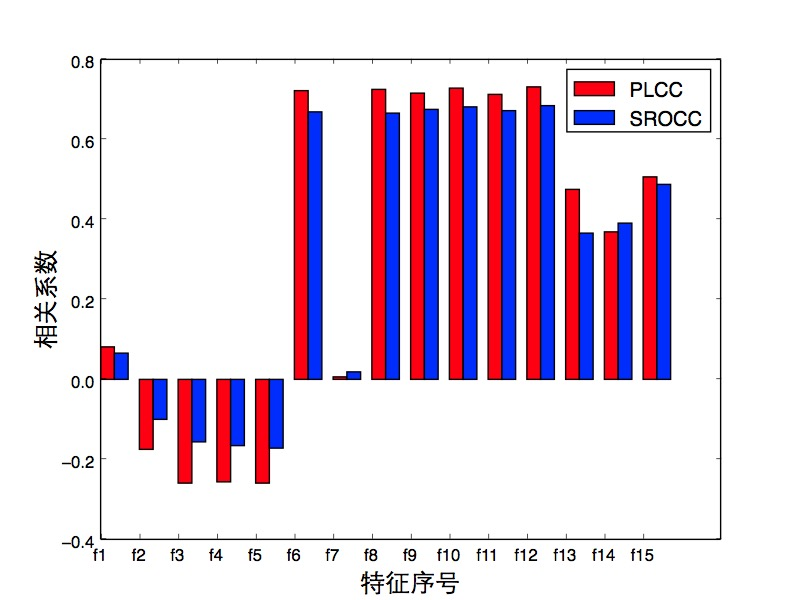
\includegraphics[width=0.75\textwidth]{chap5/correlationbetweenfeaturesandmos.jpg}
  \bicaption[fig:correlationbetweenfeaturesandmos]{各特征与MOS值的相关系数}{各特征与MOS值的相关系数}{Fig}{The relationship between feature and mos}
\end{figure}
\begin{figure}[!htp]
  \centering
  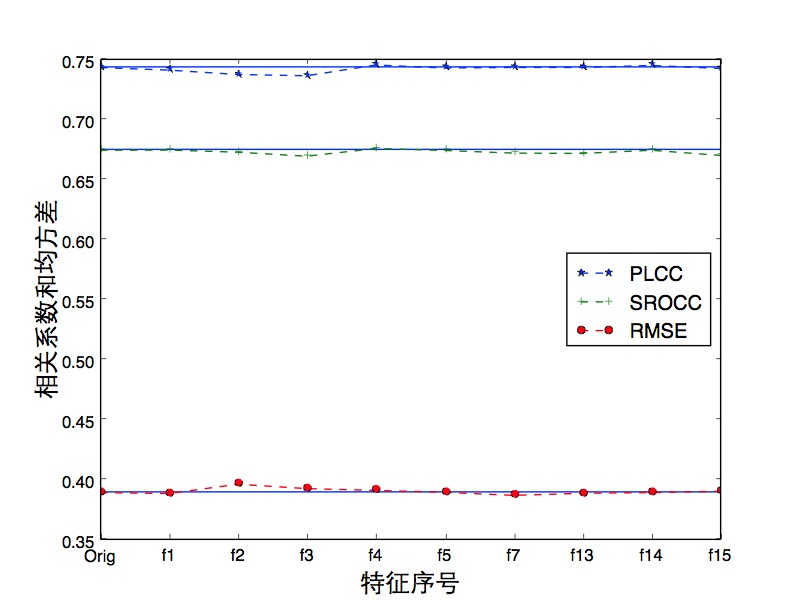
\includegraphics[width=0.78\textwidth]{chap5/validfeaturegain.jpg}
  \bicaption[fig:validfeaturegain]{验证各特征在模型中的增益}{验证各特征在模型中的增益}{Fig}{Valid the gain of each  feature}
\end{figure}
从图中可以看出:

第一,眼动数据的时序特征与空间特征与MOS值的相关度都比较低,而与视差角相关的特征与MOS值的相关度都比较高。可见,眼动数据的视差角信息是建立立体图像质量评价模型的关键。

第二,注视点和瞳孔特征都与MOS值的相关度比较低,但是也呈现出了一定的负相关性。特别地,瞳孔均值越大,图像质量越差,这与眼睛的注视生理模型是相符的------即人在注视感兴趣的事物时,瞳孔会缩小。所以瞳孔直径较大说明人眼对注视的图像没有集中聚焦,图像质量是造成这种情况的原因之一。

第三,视差角的标准差与MOS值的相关度很低。

第四,眼动的辐辏调节特征与图像质量相关,虽然没有视差角的相关度高,但是也达到了0.4以上。

经过上述讨论,我们发现在本文的特征集中,各特征与MOS的相关度不同,这些特征能否保留在模型的特征集中,现在从它们对模型效果的增益来分析。
\subsection{单个特征在模型中的增益分析}
\label{thegainoffeatures}
根据图\ref{fig:correlationbetweenfeaturesandmos},先选取相关系数最高的的特征集$\Phi '=\{f_6,f_8,f_9,f_{10},f_{11},f_{12}\}$作为基来训练,然后逐步加入其他特征,若该特征能使预测精度提升,则保留,否则,就在特征集中去掉该特征,经过测试,结果如图\ref{fig:validfeaturegain}所示:

图中Orig的位置表示只用$\Phi '$训练的结果,$f_i$位置处表示${\rm{ }}\Phi ' \cup \{ f\_i\}$ 训练的结果,从图中可以看出,特征$f_{14}$可以明显的提高模型效果,而$f_{13}$、$f_{15}$对模型的影响不大。特征$f_7$虽然与MOS的直接相关系数比较低,但是基本对模型性能没有影响。根据上述分析,我们来修正我们的模型。
\section{修正后的立体图像质量评价模型}
\label{sec:modifiedmodel}
根据\ref{sec:analysisresult}的分析,我们对各个特征对模型的增益进行了分析,并给出了各个特征对模型的影响程度。我们从整个特征集$\Phi$中剔除对模型有负影响的特征$\{f_1,f_2,f_3,f_{4},f_{5}\}$,得到新的特征集$\{f_6,f_7,...,f_{15}\}$。此时再利用算法\ref{algo:svrprocedure}来进行训练分析,最后的结果如表\ref{modifiedmodelresult}:
\begin{table}[]
\centering
\caption{修正过的模型结果}
\label{modifiedmodelresult}
\begin{tabular}{@{}cccc@{}}
\toprule
Kernel Type & PLCC              & SROCC             & RMSE             \\ \midrule
Linear      & 0.743611          & 0.673638          & \textbf{0.38614} \\
Poly        & 0.686357          & 0.67086           & 0.56813          \\
Rbf         & \textbf{0.745379} & \textbf{0.673779} & 0.387686         \\ \bottomrule
\end{tabular}
\end{table}
由于这里采用了辅眼滤波的数据特征,因此对比表\ref{svrresultbasedonnomaineye}、\ref{modifiedmodelresult}的结果如图\ref{fig:modifiedmodel.png}.
\begin{figure}[!htp]
  \centering
  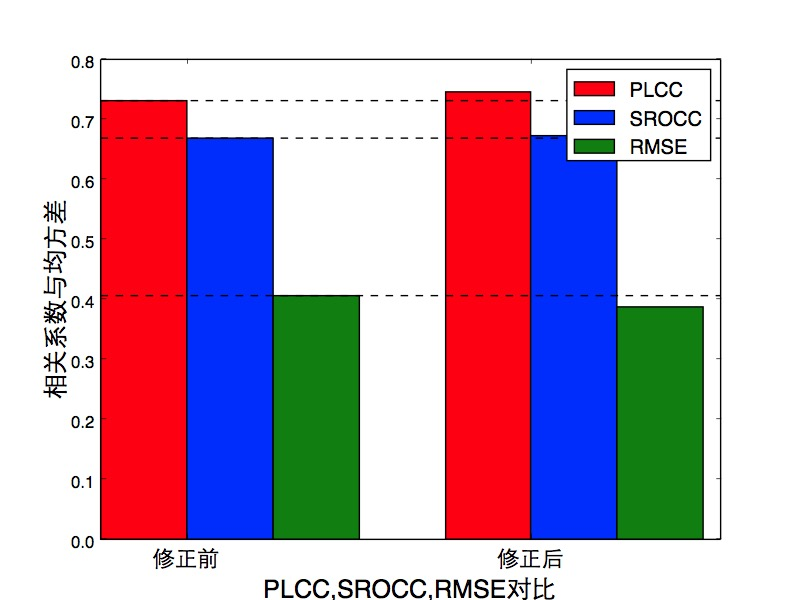
\includegraphics[width=0.75\textwidth]{chap5/modifiedmodel}
  \bicaption[fig:modifiedmodel.png]{修改前后模型效果对比图}{修改前后模型效果对比图}{Fig}{The performance of modified model}
\end{figure}
从图\ref{fig:modifiedmodel.png}我们发现,修正后的特征集在PLCC、SROCC、RMSE等三个指标上都有所提升,说明本文采用\ref{sec:analysisresult}的分析解决方法是有效的。至此,我们完成了基于眼动数据的立体图像质量评价模型。
\section{总结}
\label{sec:conclusionchapter5}
本章我们完成了基于眼动数据的立体图像质量评价模型。首先,本文给出了SVR模型的处理问题的基本流程,为后续的模型建立做好理论准备,然后基于前人研究成果和眼睛生理特征提出了15个特征,这些特征既包括眼动数据的时域和空间域的特征,也包括了利用眼动数据计算的视差角特征。其次,利用SVR建立了初步的立体图像质量评价模型,通过结果分析,得出了眼动数据特征在SVR的RBF内核函数下表现最好,且眼动数据的滤波参考眼睛应该是辅眼。再次,对各个眼动特征进行了独立验证,发现与视差角相关的特征与主观评分的相关性最高,而其他特征的表现比较差。此时采用比较好的视差角特征作为基础,对其他的特征逐个加入验证,我们发现了所有特征对模型的影响方式。最后,对模型进行了修正,剔除了对模型性能有负影响的特征,保留了正影响和几乎无影响的特征。结果表明,整体性能确实有所提升。

本章的工作证明了利用眼动数据来评价立体图像质量是可行的。我们的目的是充分利用眼动数据的特征,本文的工作可以为眼动数据特征应用提供一种新思路。
